\definecolor{roleColor}{HTML}{1F77B4}
\definecolor{skillColor}{HTML}{2CA02C}
\definecolor{responsibilityColor}{HTML}{FF7F0E}
\definecolor{benefitColor}{HTML}{9467BD}
\definecolor{companyBlurbColor}{HTML}{8C564B}
\definecolor{callToActionColor}{HTML}{D62728}
\definecolor{inclusivityColor}{HTML}{7F7F7F}
\definecolor{applicationColor}{HTML}{17BECF}

\newcommand{\legenditem}[2]{\textcolor{#2}{\rule{0.8em}{0.8em}}\hspace{0.5em}\textbf{#1}}

\chapter{Data Cleaning}
\section{Perché il Data Cleaning è necessario}

Come abbiamo visto nel capitolo precedente, gli \textit{embeddings} dei documenti ne rappresentano la \textbf{semantica}. Di conseguenza due documenti di simile significato saranno convertiti in vettori vicini.

I documenti che sono \textbf{vicini} nello spazio semantico e che si trovano in una \textbf{zona densa} di punti vengono quindi inseriti nello stesso cluster. Questo pone due importanti restrizioni nel dataset:

\begin{enumerate}
    \item I documenti devono essere \textbf{semanticamente coerenti}, poiché ogni frase inutile influisce sulla posizione del documento nello spazio semantico; di conseguenza il rumore compromette la \textbf{coerenza dei cluster}.
    \item Le frasi che riguardano argomenti non importanti per lo studio (e.g. stipendi, paragrafi legali, descrizioni aziendali, ecc.), oltre a influire sulla posizione dell'\textit{embedding} nello spazio, creano cluster non utili ai fini dell'analisi, poiché comparendo in quasi tutti i documenti generano zone dense.
\end{enumerate}

Il secondo punto è particolarmente delicato, perché cluster fittizi che raggruppano documenti in base a fattori irrilevanti non solo creano ``topic spazzatura'', cioè non informativi, ma riducono anche la sensibilità ai dettagli distintivi di un documento (e.g. mansioni, abilità richieste), sottraendo ai cluster effettivi documenti importanti.

Per visualizzare l'effetto di un data cleaning accurato confrontiamo il comportamento del modello su un dataset non preprocessato (Figura~\ref{fig:garbage-barplot}).

\begin{figure}[H]
    \centering
    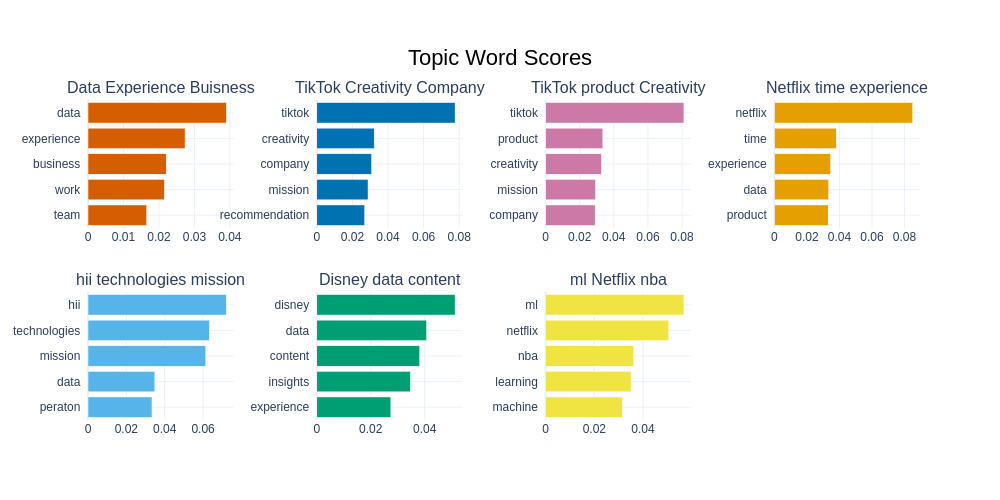
\includegraphics[width=\linewidth]{cleaning/garbage_barplot.png}
    \caption{Barplot ottenuto da \textit{topic modeling} senza \textit{preprocess}.}
    \label{fig:garbage-barplot}
\end{figure}

Come visto nel capitolo precedente, a ogni parola è associato uno \textit{score} che ne rappresenta l'importanza all'interno del topic. Questo barplot ci permette di fare alcune considerazioni importanti sulla natura del dataset e sulla direzione che deve assumere la pulizia dei dati. Innanzitutto notiamo che i nomi delle aziende, come TikTok e Netflix, hanno un peso molto grande; ciò è coerente con la natura del dataset, composto da offerte di lavoro basate negli USA, quindi è plausibile che Big Tech e altre multinazionali compaiano nella maggior parte degli annunci. Altre parole poco informative che compaiono in più topic sono legate al gergo aziendale (e.g. mission, team) e derivano dal \textit{blurb} aziendale spesso presente negli annunci. Già con queste considerazioni preliminari otteniamo un buon punto di partenza per stabilire \textbf{cosa} eliminare dal dataset.

Un buon punto di partenza, ma non sufficiente. Per capire bene cosa eliminare dobbiamo osservare i dati grezzi e comprendere meglio la natura del corpus. Riportiamo di seguito un esempio che riteniamo rappresentativo, frutto dell'analisi dei dati grezzi, che ci ha permesso di decidere quali porzioni di testo andassero rimosse e quali invece preservate.

\begin{figure}[H]
    \centering
    \scriptsize
\begin{minipage}[t]{0.47\textwidth}
    \raggedright
    \textbf{\textcolor{roleColor}{Ruolo}}\par
    We are seeking an experienced and proactive Business Intelligence Engineer or lead to join our dynamic team. As a BI Engineer, you will be responsible for [...]\par
    {\color{roleColor}\rule{\linewidth}{0.6pt}}\par\medskip

    \textbf{\textcolor{skillColor}{Abilità}}\par
    Ability to work in a fast-paced, high-energy environment and bring sense of urgency \& attention to detail skills to the table. [...] \par
    {\color{skillColor}\rule{\linewidth}{0.6pt}}\par\medskip

    \textbf{\textcolor{responsibilityColor}{Responsabilità}}\par
    Responsibilities:\par\smallskip
    ETL processes — design, develop, and maintain ETL processes using Informatica IICS (Integration Cloud Services) and IDMC (Intelligent Data Management Cloud), ensuring efficient data extraction, transformation, and loading from various source systems. [...]\par
    {\color{responsibilityColor}\rule{\linewidth}{0.6pt}}\par\medskip

    \textbf{\textcolor{benefitColor}{Benefit}}\par
    Expected salary ranges between 100,000 and 150,000 USD annually. [...]\par
    {\color{benefitColor}\rule{\linewidth}{0.6pt}}\par\medskip
\end{minipage}
\hfill
\begin{minipage}[t]{0.47\textwidth}
    \raggedright
    \textbf{\textcolor{companyBlurbColor}{Blurb aziendale}}\par
    About Regal Rexnord. Regal Rexnord is a publicly held global industrial manufacturer with 30,000 associates around the world who help create a better tomorrow [...]\par
    {\color{companyBlurbColor}\rule{\linewidth}{0.6pt}}\par\medskip

    \textbf{\textcolor{callToActionColor}{Call to action}}\par
    For more information, including a copy of our Sustainability Report, visit RegalRexnord.com.\par
    {\color{callToActionColor}\rule{\linewidth}{0.6pt}}\par\medskip

    \textbf{\textcolor{inclusivityColor}{Disclaimer su inclusività}}\par
    Equal Employment Opportunity Statement.\par\smallskip
    Regal Rexnord is an Equal Opportunity and Affirmative Action Employer. All qualified applicants will receive consideration for employment without regard to race, color, religion [...]\par
    {\color{inclusivityColor}\rule{\linewidth}{0.6pt}}\par\medskip

    \textbf{\textcolor{applicationColor}{Come inviare curriculum}}\par
    Notification to agencies:\par\smallskip
    please note that Regal Rexnord Corporation and its affiliates and subsidiaries (``Regal Rexnord'') do not accept unsolicited resumes or calls from third-party recruiters or employment agencies. [...]\par 
    {\color{applicationColor}\rule{\linewidth}{0.6pt}}\par\medskip
\end{minipage}

    \caption{Esempio annotato di annuncio di lavoro e sezioni considerate nella fase di data cleaning.}
    \label{fig:job-offer-example}
\end{figure}
\noindent Questa struttura si riscontra nella maggior parte degli annunci analizzati. I paragrafi che riteniamo cruciali per gli obiettivi dello studio sono \textit{Ruolo}, \textit{Abilità} e \textit{Responsabilità}, perché descrivono la \textbf{natura del lavoro}. Gli altri blocchi, ovvero \textit{Benefit}, \textit{Blurb aziendale}, \textit{Call to action}, \textit{Disclaimer su inclusività} e \textit{Come inviare curriculum}, costituiscono il rumore che intendiamo rimuovere. Abbiamo quindi identificato \textbf{cosa} eliminare; nella successiva sezione ci occuperemo del \textbf{come}.

\section{Divisione in paragrafi}

\noindent La suddivisione di un testo in paragrafi semanticamente coerenti è un problema aperto nella disciplina dell'\textit{nlp}, ed è stato uno dei problemi più complessi affrontati in questo studio. Un primo approccio che abbiamo tentato è stato suddividere le descrizioni degli annunci in base a segni di punteggiatura, caratteri speciali (e.g. \texttt{\textbackslash n}) e numero di parole. Il problema di questo approccio è che introduce dei metaparametri, come ad esempio numero di divisioni massime, lunghezza minima, ecc., che poco hanno a che fare con il significato del testo. Come risultato abbiamo ottenuto una divisione abbastanza omogenea nella lunghezza, ma grossolana nella coerenza semantica. Inoltre gli annunci di lavoro hanno una struttura ortografica poco coerente: qualche annuncio suddivide le informazioni con un elenco, altri separano tramite newline, altri ancora non separano affatto i paragrafi. Si è reso quindi necessario una ricerca di un' altro tipo di struttura comune, o se non altro fortemente ricorrente, nella segmentazione degli annunci.

\medskip

\noindent Studiando nuovamente il dataset abbiamo notato che molti paragrafi iniziano con un'intestazione: nell'esempio sopra possiamo notare: "Responsabilities:" e "Equal Employment Opportunity Statement". Moltissimi annunci usano questa divisione, probabilmente  per motivi di leggibilità data la lunghezza, ma non tutti; dunque abbiamo scelto la divisione basata su intestazioni come strategia principale e la vecchia strategia basata sulla punteggiatura come \textit{fallback} nel caso di paragrafi troppo lunghi, questo perché se un paragrafo è lungo è probabile che contenga frasi con significati distanti, inoltre il modello che vedremo nella sezione successiva predilige blocchi di testo con poche frasi.

\medskip
\subsubsection{Riconoscere le intestazioni}
\noindent Come riconoscere un'intestazione è più complicato di come si potrebbe pensare, un primo tentativo che abbiamo svolto utilizzava delle \textit{espressioni regolari}, ad esempio:

\begin{lstlisting}[language=python]
JOB_CUES_PAT = re.compile(
    r"(?i)\b("
    r"job\s+description|about\s+the\s+role|responsabilit|activit|"
    r"requirements?|qualifications?|what\s+you'll\s+(do|be\s+doing)|"
    r"skills|nice\s+to\s+have|profilo"
    r")\b"
)
\end{lstlisting}

\noindent Però le regex si sono rivelate troppo rigide allo scopo, ad esempio un intestazione tipo "At Google you will:" non verrebbe catturata.

\medskip

\noindent Un altro tentativo è stato quello di selezionare le righe che fossero composte da massimo n parole o che terminassero con un carattere \textit{":"}, chiaramente anche questo tentativo è risultato fallimentare poiché alcune intestazioni si rivelano ben più lunghe di quanto si potrebbe immaginare, mentre altre frasi brevi potrebbero essere confuse per intestazioni. Dunque ci serve un metodo che sia sufficentemente flessibile, per questo abbiamo scelto di addestrare una rete neurale.

\medskip

\noindent La libreria scelta per l'addestramento è \textit{Spacy}.

\medskip

\subsection{Spacy}
\noindent Spacy è una libreria per \textit{nlp} basata su \textit{pipelines} composte da moduli modificabili e allenabili. Questa componente altamente personalizzabile della libreria la rende ideale per il nostro studio, infatti in momenti diversi utilizzeremo componenti differenti a seconda del bisogno.

\noindent Le \textit{pipelines} elaborano un testo e restituiscono un \textit{Doc}, un oggetto che permette di accedere alle informazioni del testo ottenute dalla pipeline. Un Doc è una sequenza di Python composta da \textit{token}. In spacy i token sono parole o segni di punteggiatura.
\noindent Gli \textit{span} invece sono sottosequenze del documento, composte da token contigui.

\begin{lstlisting}[language=python]
nlp = spacy.blank("en")     # Creazione pipeline default
doc = nlp("Hello world!")

for token in doc:
    print(token.text)
\end{lstlisting}

\noindent \textbf{Output:}

\begin{lstlisting}[style=output]
Hello
world
!
\end{lstlisting}

\begin{lstlisting}[language=python]
span = doc[1:3]
print(span.text)
\end{lstlisting}

\noindent \textbf{Output:}

\begin{lstlisting}[style=output]
world!
\end{lstlisting}

\noindent I moduli della pipeline lavorano salvando le informazioni sui token, sugli span o sul Doc. Uno dei moduli custom allenabili è lo SpanCategorizer (spancat in breve) che permette di riconoscere ed etichettare span.\footnote{\url{https://spacy.io/api/spancategorizer}} Possiamo quindi interpretare le intestazioni come \textit{span} e allenare un modello per riconoscerle. Lo spancat è composto da due parti:
\begin{enumerate}
    \item Funzione \textit{suggester}, che indica quali span sono candidati alla categorizzazione.
    \item Rete neurale responsabile della classificazione, suddivisa in più sottoreti
\end{enumerate}

\noindent Per configurare il modello (e l'allenamento), spaCy richiede un file \texttt{config.cfg}, vediamo adesso il suggester e tutte le componenti della rete neurale.
\subsubsection{Suggester}
Il \textit{Suggester} utilizzato è quello di default, \texttt{spacy.ngram\_suggester.v1}, che marca come candidati tutti gli span possibili entro una certa lunghezza.

\begin{figure}[H]
    \centering
    \scriptsize
\begin{lstlisting}[style=cmd]
[components.spancat.suggester]
@misc = "spacy.ngram_suggester.v1"
sizes = [1,2,3,4,5,6,7,8,9,10,11,12,13,14,15,16,17,18,19,20]
\end{lstlisting}
    \caption{Configurazione del \textit{suggester}: usa il componente \texttt{spacy.ngram\_suggester.v1} e valuta tutti gli span fino a 20 token per coprire la varietà degli header.}
    \label{fig:cfg-suggester}
\end{figure}

\noindent Ho impostato 20 come lunghezza massima a causa della varietà degli header: il modello risulta molto flessibile, ma anche più pesante, perché all'aumentare degli n-grammi possibili aumentano i controlli da effettuare.
Vediamo adesso come è composta la rete neurale, partendo dalla sua prima componente: \textbf{Tok2Vec}.
\subsubsection{Tok2Vec}
\noindent È suddiviso in due sottoreti embedder ed encoder. L'\textit{embedder} converte i token in vettori ignorando il contesto.

\begin{figure}[H]
    \centering
    \scriptsize
\begin{lstlisting}[style=cmd]
[components.tok2vec.model.embed]
@architectures = "spacy.MultiHashEmbed.v2"
width = 96
attrs = ["NORM","PREFIX","SUFFIX","SHAPE"]
rows = [5000,1000,2500,2500]
include_static_vectors = false
\end{lstlisting}
    \caption{Configurazione dell'\textit{embedder}: vettori da 96 dimensioni con attributi morfologici distinti (\texttt{NORM}, \texttt{PREFIX}, \texttt{SUFFIX}, \texttt{SHAPE}) e hash table calibrate su 5000/1000/2500/2500 voci; gli embedding esterni non vengono usati.}
    \label{fig:cfg-embed}
\end{figure}

\noindent Gli attributi indicano quali caratteristiche del token contribuiscono all'embedding e forniscono alla rete informazioni morfologiche e ortografiche utili per riconoscere pattern linguistici: \texttt{NORM} è la parola normalizzata (senza maiuscole, accenti o varianti equivalenti, e.g. \texttt{'s} diventa \texttt{is}); \texttt{PREFIX} e \texttt{SUFFIX} sono autoesplicativi; \texttt{SHAPE} descrive la forma ortografica (\texttt{Data}: \texttt{Xxxx}, \texttt{NASA}: \texttt{XXXX}, \texttt{2025}: \texttt{dddd}). Il componente \texttt{MultiHashEmbed.v2} crea embedding separati per ciascun attributo,\footnote{\url{https://spacy.io/api/architectures\#MultiHashEmbed}} così ogni token è rappresentato dal significato, dalla forma ortografica e da porzioni specifiche della parola. In \texttt{rows} impostiamo la dimensione massima della tabella hash per ogni attributo; trattandosi di matrici che associano a ciascun valore un vettore, abbiamo dimensionato le tabelle in base alla varietà attesa degli attributi, prevedendo ad esempio molte più forme normalizzate rispetto ai prefissi e rimanendo entro il bound consigliato (1000--10000).

\noindent L'\textit{encoder} modifica i vettori in funzione del \textit{contesto}.

\begin{figure}[H]
    \centering
    \scriptsize
\begin{lstlisting}[style=cmd]
[components.tok2vec.model.encode]
@architectures = "spacy.MaxoutWindowEncoder.v2"
width = 96
depth = 4
window_size = 1
maxout_pieces = 3
\end{lstlisting}
    \caption{Encoder \texttt{MaxoutWindowEncoder}: stesso spazio vettoriale a 96 dimensioni, quattro strati con finestra contestuale di un token per lato e tre proiezioni Maxout per modellare non linearità.}
    \label{fig:cfg-encode}
\end{figure}

\noindent I vettori vengono processati da una rete \textit{feed-forward}: ogni strato calcola tre proiezioni lineari e applica \textit{Maxout}, scegliendo quella con valore massimo per ogni finestra. L'uso di \textit{Maxout}, al posto di una semplice ReLU, permette di modellare dipendenze contestuali più complesse.
\subsubsection{Reducer}

\noindent Questo componente sintetizza uno span in un unico vettore di dimensione \texttt{hidden\_size}.

\begin{figure}[H]
    \centering
    \scriptsize
\begin{lstlisting}[style=cmd]
[components.spancat.model.reducer]
@layers = "spacy.mean_max_reducer.v1"
hidden_size = 128
\end{lstlisting}
    \caption{Reducer \texttt{mean\_max}: combina media e massimo dei token in un vettore di dimensione 128 prima dello strato di scoring.}
    \label{fig:cfg-reducer}
\end{figure}

\noindent Il componente \texttt{MeanMaxReducer} calcola la media dei token, il massimo dei token e concatena i due vettori in un'unica rappresentazione, sulla quale applica un \textit{hidden layer}; la documentazione indica la presenza del layer ma non ne esplicita la struttura.\footnote{\url{https://spacy.io/api/architectures\#mean\_max\_reducer}}
\subsubsection{Scorer}

\noindent Il layer finale mappa il vettore dello span sulla probabilità di classe, utilizzando una funzione di attivazione \textbf{sigmoide}.

\begin{figure}[H]
    \centering
    \scriptsize
\begin{lstlisting}[style=cmd]
[components.spancat.model.scorer]
@layers = "spacy.LinearLogistic.v1"
nO = 1
nI = null
\end{lstlisting}
    \caption{Scorer logistico lineare: un'unica uscita sigmoide (\texttt{nO = 1}) alimentata dal vettore di dimensione 128 prodotto dal reducer.}
    \label{fig:cfg-scorer}
\end{figure}
Il layer usato qui è uno strato lineare seguito da una \textbf{sigmoide}.
Poiché SBERT (usato per la classificazione dei paragrafi) predilige documenti composti da poche frasi, e per limitare il numero di paragrafi spuri (cioè che comprendono informazioni di classi diverse), abbiamo scelto 0.2 come probabilità minima per classificare uno span come header, in modo da avere una segmentazione più fine.
Il contro di questo approccio è che se il documento è troppo corto SBERT non ha il contesto necessario per fare una classificazione robusta, parleremo del problema nella sezione relativa al \textit{fallback}.

\subsubsection{Allenamento}

\noindent Come detto in precedenza il file \textit{config.cfg} definisce anche l'allenamento della rete. Il \textit{corpus} è composto da 149 descrizioni selezionate inizialmente a caso dal dataset completo, poi a causa della comparsa di numerosi annunci dalla stessa azienda abbiamo deciso di sostituire alcuni annunci della suddetta con altri che mai comparivano nei 149 estratti, questo per evitare overfitting e migliorare la capacità del modello di generalizzare. In queste descrizioni abbiamo individuato 1083 intestazioni.

\noindent Abbiamo quindi suddiviso il corpus in \textit{train} usato per l'allenamento e \textit{dev} usato per la valutazione. la grandezza del \textit{dev set} è del 10\% del corpus, siamo consci del fatto che sia una porzione di dati troppo esigua per avere delle valutazioni statistiche robuste, cionondimeno abbiamo deciso volutamente di creare una disparità in favore del training set poiché il modello è composto da più strati, tutti da allenare (embedder, encoder, reducer e scorer), dunque abbiamo evitato di sottrarre informazioni utili all'apprendimento. Vediamo adesso nello specifico come è impostato il training:

\begin{figure}[H]
    \centering
    \scriptsize
\begin{lstlisting}[style=cmd]
[training]
dev_corpus = "corpora.dev"
train_corpus = "corpora.train"
seed = ${system.seed}
gpu_allocator = ${system.gpu_allocator}
dropout = 0.1
accumulate_gradient = 1
patience = 1600.
L'F-score rimane buono in entrambi i casi, questo vuol dire che il modello generalizza bene, anche se perde qualche intestazione marginale.
max_epochs = 0
max_steps = 20000
eval_frequency = 200
\end{lstlisting}
    \caption{Parametri di training: dropout fissato a 0.1, aggiornamento dopo ogni batch (\texttt{accumulate\_gradient = 1}), early stopping con \texttt{patience} 1600 valutazioni e \texttt{max\_steps} 20000; valutazione sul dev ogni 200 step.}
    \label{fig:cfg-training}
\end{figure}

\noindent Il corpo viene suddiviso in batch di grandezza variabile, i batch non sono composti da documenti, ma da token, per migliorare le performance quando l'allenamento avviene su GPU. A ogni passo di training, la dimensione del batch viene moltiplicata per un fattore 1.001, partendo da 100 token fino a un massimo di 1000; in questo modo batch piccoli vengono usati all'inizio del training, per avere gradienti più rumorosi ma anche più esplorativi, man mano che il training prosegue si prediligono batch sempre più grandi per avere gradienti più stabili e precisi. \textit{Nota: valutare se inserire info riguardo l'ottimizzatore che è Adam.}

\subsection{Valutazione del modello}

\begin{figure}[H]
    \centering
    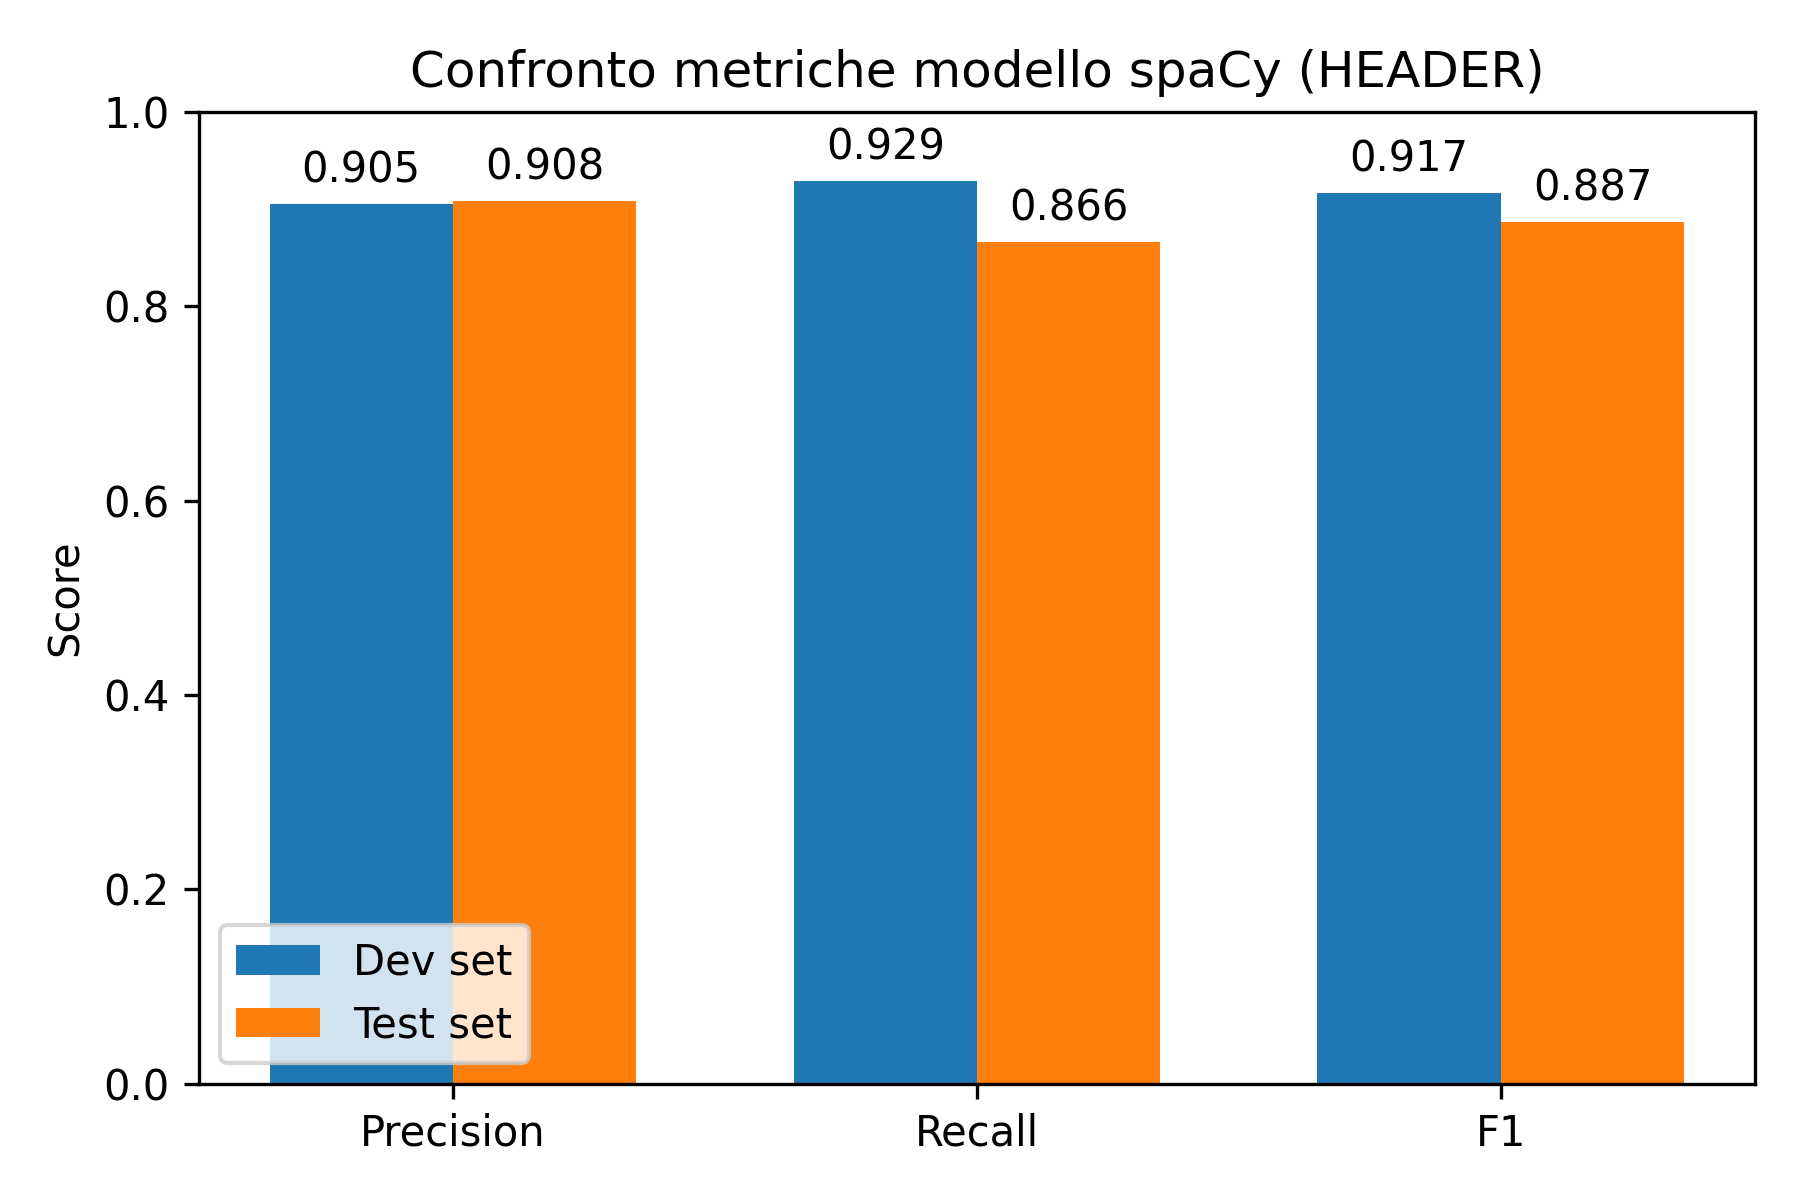
\includegraphics[width=0.75\linewidth]{cleaning/header_metrics_comparison.png}
    \caption{Confronto delle metriche \textit{precision}, \textit{recall} e \textit{F-score} tra la valutazione fatta nel dev set e quella nel test set.}
    \label{fig:header-metrics}
\end{figure}

\noindent Il \textit{test set} è composto da altre 20 descrizioni per un totale di 150 intestazioni.
\noindent Il modello mostra una \textit{precisione} elevata e una \textit{sensibilità} complessivamente soddisfacente. La \textit{recall}, come evidenziato in Figura~\ref{fig:header-metrics}, diminuisce in modo sensibile, ma rimane entro un intervallo accettabile per l'obiettivo di segmentazione. L'\textit{F-score} resta stabile e su valori buoni, a indicare che la rete generalizza bene: qualche intestazione marginale viene persa, ma il bilanciamento tra falsi positivi e falsi negativi rimane favorevole.
\subsection{Fallback}

\noindent Come affermato in precedenza, abbiamo implementato una strategia di \textit{fallback} per suddividere i paragrafi troppo lunghi. Il primo approccio testato è stato quello di utilizzare la \textit{cosine similarity} fra frasi:
\begin{enumerate}
    \item si divide il paragrafo in frasi;
    \item si calcola l'embedding di ogni frase con SBERT;
    \item a partire dalla seconda frase si misura la \textit{cosine similarity} con quella precedente e, quando scende sotto soglia, si spezza il paragrafo.
\end{enumerate}
\noindent In teoria il metodo avrebbe dovuto raggruppare frasi semanticamente affini e separare cambi di argomento. In pratica, molti paragrafi omogenei presentavano similarità basse e, in generale, la \textit{similarità tra frasi} non risultava abbastanza correlata al cambio di argomento. Siamo quindi tornati a una suddivisione più ortografica basata su soglie di lunghezza (in termini di \textit{token} spaCy), numero minimo di frasi e doppi \texttt{\textbackslash n\textbackslash n}.

\begin{figure}[H]
    \centering
    \scriptsize
\begin{lstlisting}[language=python]
nlp_sent = spacy.blank("en")
nlp_sent.add_pipe("sentencizer")

def count_sentences(part: str) -> int:
    doc = nlp_sent(part)
    return len(list(doc.sents))

def _split_long_paragraph(span, max_tokens=120, min_sents=2):
    text = span.text
    if len(span) < max_tokens:
        return [text]

    parts = [p.strip() for p in text.split("\n\n") if p.strip()]
    buffer = ""
    paragraphs = []

    for i, part in enumerate(parts):
        n_sents = count_sentences(part)
        if n_sents <= min_sents and i < len(parts) - 1:
            buffer += "\n" + part
        else:
            paragraphs.append((buffer + "\n" + part).strip())
            buffer = ""

    if buffer:
        paragraphs.append(buffer.strip())

    return paragraphs
\end{lstlisting}
    \caption{Funzione di fallback: sfrutta i token e il modulo \texttt{sentencizer} di spaCy (all'interno di \texttt{count\_sentences}) per riconoscere le frasi in un blocco di testo.}
    \label{fig:fallback-split}
\end{figure}

\noindent L'euristica divide il testo sugli \texttt{\textbackslash n\textbackslash n}, accumula i blocchi troppo corti in un buffer e restituisce sotto-paragrafi con almeno due frasi e meno di 120 token, così SBERT riceve segmenti informativi senza perdere il contesto.
L'uso di una doppia strategia garantisce una buona granularità nella suddivisione del testo, infatti annunci in cui non sono presenti né intestazioni, né doppi new line sono pochi e hanno quindi un peso basso in BERTopic.
\section{Classificazione paragrafi}

\noindent Una volta completata la divisione in paragrafi, analizziamo come abbiamo affrontato la classificazione. Dobbiamo gestire testi di lunghezza variabile ma comunque limitati a poche frasi. Abbiamo deciso di utilizzare un modello della libreria \textit{Sentence Transformers} per creare gli embedding dei paragrafi, a cui abbiamo poi applicato un layer di \textit{Logistic Regression} che classifica gli embedding. Anche in questo caso abbiamo adottato \textit{all-mpnet-base-v2}, poiché fornisce embedding semantici di alta qualità, come visto nel capitolo precedente.

\subsection{Etichettatura}

\noindent Il primo step per l'allenamento del modello è creare il \textit{training set} e il \textit{test set}. Un test preliminare è stato effettuato etichettando 178 paragrafi con 10 etichette diverse; di seguito riportiamo le etichette con il relativo numero di paragrafi:

\begin{center}
\begin{tabular}{ll}
\textbf{JOB} & 91 \\
\textbf{BLURB} & 25 \\
\textbf{BENEFIT} & 23 \\
\textbf{DEI} & 15 \\
\textbf{LEGAL} & 10 \\
\textbf{LOCATION} & 5 \\
\textbf{SCHEDULE} & 3 \\
\textbf{CONTRACT} & 3 \\
\textbf{CALL TO ACTION} & 2 \\
\textbf{HOW TO APPLY} & 1 \\
\end{tabular}
\end{center}

\noindent In particolare, \textbf{JOB} contiene i paragrafi che abbiamo precedentemente identificato con ``Ruolo'', ``Abilità'' e ``Responsabilità''; \textbf{DEI} include i paragrafi dedicati alle politiche di inclusione ed equità; \textbf{LEGAL} raggruppa i disclaimer legali; \textbf{CONTRACT} raccoglie le specifiche burocratiche del contratto.

\noindent Come è facile notare solo la classe \textbf{JOB} risulta ben rappresentata; le uniche altre due classi con un numero sufficiente di esempi sono \textbf{BLURB} e \textbf{BENEFIT}. Per questo motivo abbiamo deciso di fondere le classi sottorappresentate, così da evitare un crollo delle performance sulle classi più piccole. La scelta della fusione è ricaduta su due opzioni alternative:

\begin{enumerate}
    \item \textbf{Binario semplice}
    \item \textbf{Multi-classe intermedia}
\end{enumerate}

\noindent Il binario semplice risolve il problema della sotto-rappresentazione, ma rischia di generalizzare peggio poiché le classi \textbf{JOB} e \textbf{NON-JOB} risultano molto eterogenee. Il multi-classe, invece, aiuta SBERT a strutturare meglio lo spazio semantico; di contro richiede più dati per garantire una rappresentazione adeguata di tutte le classi. Abbiamo quindi optato per il multi-classe, incrementando significativamente la dimensione del \textit{training set} per ottenere un addestramento più stabile.

\noindent Le classi finali adottate sono tre:

\begin{itemize}
    \item \textbf{JOB}: come definita precedentemente.
    \item \textbf{BLURB-LEGAL}: unione di blurb, DEI, legal, call to action e how to apply.
    \item \textbf{OFFER-DETAIL}: unione di benefit, location, schedule, contract.
\end{itemize}

\noindent Useremo dunque più classi in fase di addestramento, ma il modello verrà impiegato come classificatore binario scartando le classi diverse da \textbf{JOB}. Il \textit{dataset} finale è composto da 1315 paragrafi così etichettati:

\begin{center}
\begin{tabular}{ll}
\textbf{JOB} & 700 \\
\textbf{BLURB-LEGAL} & 340 \\
\textbf{OFFER-DETAIL} & 275 \\
\end{tabular}
\end{center}

\noindent Lo sbilanciamento a favore di \textbf{JOB} potrebbe apparire problematico: quando le classi sono sbilanciate un classificatore tende a privilegiare la classe maggioritaria, con il rischio di introdurre un \textit{bias} verso \textbf{JOB}. Tuttavia il nostro obiettivo è pulire il dataset \textit{evitando di tagliare informazioni potenzialmente rilevanti} per lo studio; di conseguenza, nel caso in cui il modello fosse incerto, è preferibile preservare il paragrafo per non eliminare contenuti importanti. In quest'ottica avere un'unica classe \textbf{JOB} (anziché distinguere Ruolo, Abilità e Responsabilità) può rivelarsi un vantaggio. Questa politica di ``favoritismo'' verso la classe \textbf{JOB} verrà riutilizzata sia nel training dell'embedder sia nelle politiche di cancellazione dei paragrafi post-classificazione, come illustrato nelle sezioni successive.
\subsubsection{Allenamento}

\begin{figure}[H]
    \centering
    \scriptsize
\begin{lstlisting}[language=python]
X_train, X_test, y_train, y_test = train_test_split(
    df["text"],
    df["label"],
    test_size=0.2,
    stratify=df["label"],
    random_state=10,
)
\end{lstlisting}
    \caption{Il 20\% del dataset è usato come test set per la valutazione. L'opzione \texttt{stratify=df["label"]} preserva la distribuzione delle classi tra train e test, indispensabile in presenza di classi sbilanciate.}
    \label{fig:clf-split}
\end{figure}

\noindent Dopo la suddivisione del dataset e la creazione e normalizzazione degli embedding resta la classificazione effettiva, le opzioni che abbiamo preso in considerazione sono:

\begin{enumerate}
    \item \textbf{Rete neurale}
    \item \textbf{Fine-tuning del transformer}
    \item \textbf{Logistic Regression}
\end{enumerate}

\noindent Una rete neurale può apprendere relazioni non lineari tra gli embedding per catturare interazioni più complesse. Questo approccio può ottenere buone prestazioni in presenza di dataset di dimensioni maggiori, comporta inoltre una maggiore complessità di addestramento e un rischio più elevato di overfitting rispetto a modelli lineari.

\noindent Con \textit{fine tuning del transformer} intendiamo il riaddestramento parziale (cioè solo degli ultimi layer) del modello Transformer stesso, aggiungendo in coda al modello una piccola testa di classificazione. Questa strategia offre un grande vantaggio in più rispetto alla precedente: l'adattamento al dominio. Infatti SBERT non sarebbe più un generatore di embedding statici, ma coglierebbe sfumature linguistiche specifiche degli annunci di lavoro, riducendo l’ambiguità tra frasi che nei dati generali erano simili, ma nel dominio degli annunci hanno significati distinti; questo potrebbe aumentare sensibilmente la capacità del modello di discriminare più accuratamente paragrafi simili. Chiaramente un approccio del genere richiederebbe un dataset di dimensioni ben maggiori, con almeno alcune migliaia di esempi. Abbiamo comunque ritenuto importante menzionarlo per eventuali sviluppi futuri.

\noindent L'opzione scelta è quindi la \textbf{Logistic Regression}, che è adatta alla dimensione del nostro dataset, con basso rischio di overfitting rispetto alle scelte precedenti; inoltre gli embedding di \textit{all-mpnet-base-v2} sono già molto informativi, anche senza \textit{fine tuning}, quindi LR deve solo apprendere frontiere di decisione lineari, non estrarre feature dal testo grezzo.

\begin{figure}[H]
    \centering
    \scriptsize
\begin{lstlisting}[language=python]
clf = LogisticRegression(
    max_iter=2000,
    class_weight={"JOB": 1.5, "BLURB": 1.0, "DETAIL": 1.0},
    random_state=10,
)
\end{lstlisting}
    \caption{Configurazione del classificatore LR: massimo 2000 iterazioni, pesi maggiorati per la classe \texttt{JOB} (1.5) e bilanciamento minore per \texttt{BLURB} e \texttt{DETAIL}.}
    \label{fig:clf-lr}
\end{figure}

La \textit{class weight} rappresenta il peso che ha una classe nella funzione di \textit{loss}. Aumentando il peso di una classe il modello riceve gradienti più forti durante la \textit{backpropagation} e impara quindi a classificarla meglio. Abbiamo prediletto pesi maggiori per \textbf{JOB} per le ragioni espresse nella sezione precedente. I valori testati per la \textit{class weight} di \textbf{JOB} sono 1.0, 1.5 e 2.0; i risultati principali sono riassunti in Figura~\ref{fig:lr-reports}.

\begin{figure}[H]
    \centering
    \scriptsize
    \begin{tabular}{@{}p{0.45\textwidth}@{\hspace{1em}}p{0.45\textwidth}@{}}
        \multicolumn{2}{c}{\textbf{Balanced (1.0)}}\\[0.4em]
        \begin{tabular}{lccc}
        & \textbf{Prec.} & \textbf{Rec.} & \textbf{F1} \\
        DETAIL & 0.87 & 0.93 & 0.90 \\
        BLURB & 0.85 & 0.90 & 0.88 \\
        JOB & 0.97 & 0.92 & 0.94 \\
        \end{tabular} &
        $\begin{array}{c|ccc}
            & \textbf{DET.} & \textbf{BLURB} & \textbf{JOB} \\
            \hline
            \textbf{DET.} & 253 & 13 & 7 \\
            \textbf{BLURB} & 20 & 306 & 13 \\
            \textbf{JOB} & 18 & 41 & 637 \\
        \end{array}$\\[1em]
        \multicolumn{2}{c}{\textbf{Slightly unbalanced (1.5)}}\\[0.4em]
        \begin{tabular}{lccc}
        & \textbf{Prec.} & \textbf{Rec.} & \textbf{F1} \\
        DETAIL & 0.91 & 0.85 & 0.88 \\
        BLURB & 0.89 & 0.81 & 0.85 \\
        JOB & 0.91 & 0.97 & 0.94 \\
        \end{tabular} &
        $\begin{array}{c|ccc}
            & \textbf{DET.} & \textbf{BLURB} & \textbf{JOB} \\
            \hline
            \textbf{DET.} & 231 & 22 & 20 \\
            \textbf{BLURB} & 16 & 275 & 48 \\
            \textbf{JOB} & 8 & 13 & 675 \\
        \end{array}$\\[1em]
        \multicolumn{2}{c}{\textbf{Unbalanced (2.0)}}\\[0.4em]
        \begin{tabular}{lccc}
        & \textbf{Prec.} & \textbf{Rec.} & \textbf{F1} \\
        DETAIL & 0.91 & 0.84 & 0.88 \\
        BLURB & 0.89 & 0.80 & 0.85 \\
        JOB & 0.90 & 0.97 & 0.94 \\
        \end{tabular} &
        $\begin{array}{c|ccc}
            & \textbf{DET.} & \textbf{BLURB} & \textbf{JOB} \\
            \hline
            \textbf{DET.} & 230 & 20 & 23 \\
            \textbf{BLURB} & 15 & 272 & 52 \\
            \textbf{JOB} & 7 & 12 & 677 \\
        \end{array}$\\
    \end{tabular}
    \caption{Metriche di valutazione e matrici di confusione al variare del peso assegnato alla classe \textbf{JOB} nella \textit{Logistic Regression}.}
    \label{fig:lr-reports}
\end{figure}
Il modello bilanciato è quello con un \textit{f-score} più alto, però il nostro obiettivo rimane massimizzare la \textit{recall} di JOB, in cui il modello leggermente sbilanciato è più forte al netto di un leggero peggioramento nelle altre classi (atteso) e nella precisione.
Il modello più sbilanciato non offre un miglioramento della \textit{recall}, ma solo un peggioramento della performance generale del modello.
Dunque la scelta è ricaduta sul modello \textbf{Slightly unbalanced}.
\subsubsection{Strategia di rimozione}
Adesso abbiamo la probabilità di appartenenza ad una classe per ciascun paragrafo, dobbiamo scegliere come eliminare i paragrafi non informativi in base a queste informazioni:
\noindent Per mitigare i casi borderline abbiamo definito un filtro euristico che riassegna la classe finale sulla base delle probabilità restituite dal classificatore.

\begin{figure}[H]
    \centering
    \scriptsize
\begin{lstlisting}[language=python]
dominant = df[["prob_job", "prob_blurb_legal", "prob_offer_detail"]] \
    .idxmax(axis=1).str.replace("prob_", "", regex=False)
top_probs = df[["prob_job", "prob_blurb_legal", "prob_offer_detail"]].max(axis=1)

cond_blurb = df["prob_blurb_legal"] > blurb_threshold
cond_job = df["prob_job"] > job_threshold
cond_diff = (top_probs - df["prob_job"] < diff_threshold)
cond_low = top_probs < low_conf_threshold

prediction = np.select(
    [
        cond_blurb & ~cond_job,               # blurb forte e non job
        cond_job | cond_diff | cond_low       # se job, simile a job, o incerto
    ],
    ["blurb_legal", "job"],
    default=dominant                          # altrimenti usa la classe dominante
)
\end{lstlisting}
    \caption{Logica di post-processing per l'assegnazione finale della classe del paragrafo.}
    \label{fig:lr-postprocess}
\end{figure}

\noindent Cosa fa questo codice:
\begin{enumerate}
    \item un paragrafo viene etichettato come \textbf{blurb legal} solo quando la probabilità relativa supera la soglia e quella di \textbf{JOB} rimane sotto il limite stabilito; questo perché i paragrafi che più inquinano sono quelli delle descrizioni aziendali.
    \item i paragrafi con alta confidenza su \textbf{JOB}, con probabilità simile a \textbf{JOB} o complessivamente ambigui (\textit{low conf}) vengono classificati come \textbf{JOB};
    \item in tutti gli altri casi si ricorre alla classe dominante (\textit{default}) proposta dal modello.
\end{enumerate}
\section{Altre strategie di data cleaning usate}

\noindent Dopo la pulizia a livello di paragrafo analizziamo l'effetto su BERTopic. La Figura~\ref{fig:half-cleaning} mostra il dendrogramma ottenuto con il dataset parzialmente pulito.

\begin{figure}[H]
    \centering
    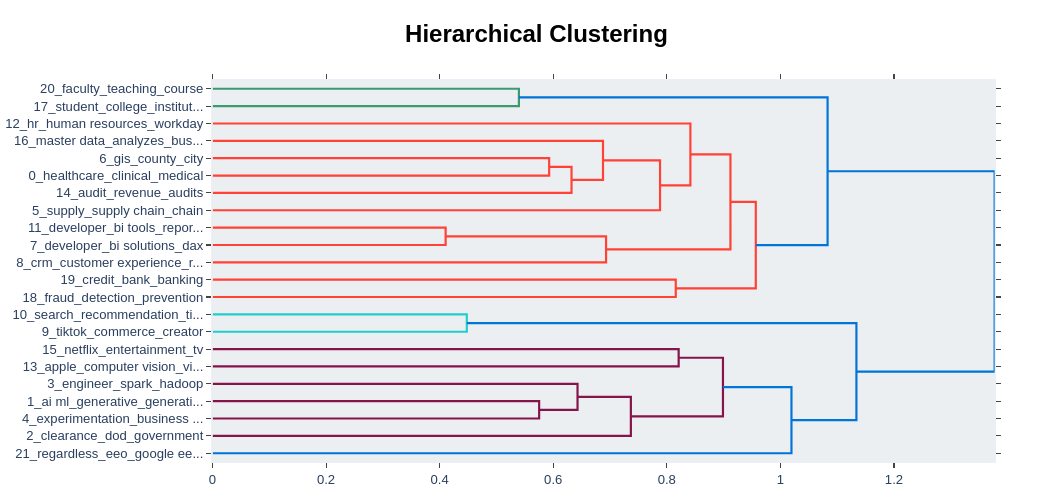
\includegraphics[width=\linewidth]{cleaning/gerarchia_half_cleaning.png}
    \caption{Dendrogramma di BERTopic su dataset parzialmente pulito.}
    \label{fig:half-cleaning}
\end{figure}

\noindent Il miglioramento rispetto al dataset grezzo è evidente, ma persistono ancora numerosi \textbf{nomi aziendali} e \textbf{luoghi}. Ciò dipende sia dalla strategia conservativa adottata in classificazione (preferire \textbf{JOB} anziché rischiare falsi negativi), sia da paragrafi misti: frasi come ``At Apple we are looking for a Data Analyst'' contengono informazioni cruciali sul ruolo, ma introducono anche riferimenti non utili.

\noindent Diventa quindi necessario affiancare alla pulizia per paragrafi una pulizia \textbf{interna alle singole frasi}, così da eliminare riferimenti ad aziende e località e permettere a BERTopic di pesare maggiormente mansioni e competenze.

\subsubsection{Pulizia tramite NER}

\noindent Per raggiungere questo obiettivo integriamo nella pipeline spaCy un componente \textit{NER} (Name Entity Recognizer) già addestrato che identifica \textit{entità} testuali (aziende, persone, stati, ecc.). I token corrispondenti a entità non informative vengono rimossi dalle frasi dei paragrafi \textbf{JOB}.

\begin{figure}[H]
    \centering
    \scriptsize
\begin{lstlisting}[language=python]
def remove_entities(texts, removable_entities={"ORG", "PERSON", "GPE"}):
    cleaned = []
    for doc in ner_model.pipe(texts):
        tokens = []
        for token in doc:
            if token.ent_type_ in removable_entities \
                    and token.text.lower() not in TECH_WHITELIST:
                continue
            tokens.append(token.text_with_ws)
        cleaned.append("".join(tokens).strip())
    return cleaned
\end{lstlisting}
    \caption{Euristica di rimozione delle entità: \texttt{ORG} identifica le organizzazioni (incluse le aziende), \texttt{GPE} le entità geopolitiche (stati, città).}
    \label{fig:ner-cleaning}
\end{figure}

\noindent In parallelo manteniamo una \textbf{whitelist} di termini tecnici (ad esempio \textit{Oracle}, \textit{GitHub}) per evitare di rimuovere entità che rappresentano competenze o strumenti rilevanti.

\subsubsection{Risultato finale}

\noindent Applicando anche questa pulizia intra-frasi otteniamo il dendrogramma della Figura~\ref{fig:cleaned-dendrogram} tramite BERTopic.

\begin{figure}[H]
    \centering
    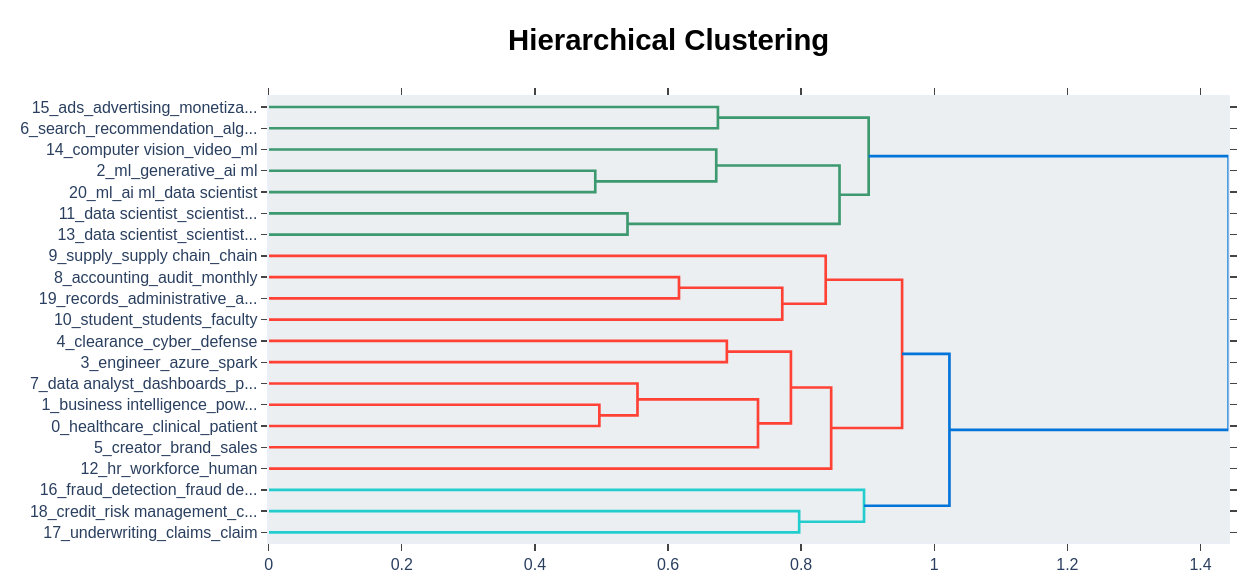
\includegraphics[width=\linewidth]{cleaning/dendrogramma_pulito.png}
    \caption{Dendrogramma di BERTopic su dataset completamente pulito.}
    \label{fig:cleaned-dendrogram}
\end{figure}

\noindent I riferimenti a \textbf{brand} e \textbf{luoghi statunitensi} scompaiono quasi del tutto e l'attenzione si concentra su mansioni, competenze e requisiti realmente utili per l'analisi del mercato del lavoro.
\section{Possibili miglioramenti}
Analizziamo quì i punti critici che potrebbero essere migliorati e speculiamo su quali altre strategie potrebbero essere attuate in uno sviluppo successivo dello studio:

